\section{Υλοποίηση}
\label{chapImplementation}

Στο παρόν κεφάλαιο βρίσκεται ο πυρήνας της εργασίας μας. Αρχικά γίνεται η παρουσίαση των εργαλείων, στα οποία βασίστηκε η υλοποίησή μας, ενώ στη συνέχεια παρατίθενται οι μέθοδοι κατανομής και παραλληλοποίησης, του αλγορίθμου απαρίθμησης Schnorr και Euchner. Τέλος, εκτίθεται το εργαλείο που αναπτύχθηκε στα πλαίσια της εργασίας, με σκοπό την προσομοίωση της κατανεμημένης λειτουργίας υλοποίησης. 

\subsection{Τεχνολογίες και μέθοδοι υλοποίησης}

\subsubsection{Γενικά χαρακτηριστικά}

Η ανάπτυξη της εργασίας καθορίστηκε από δύο παράγοντες. Ο πρώτος ήταν η ταχύτητα εκτέλεσης, ενώ ο δεύτερος, η ευκολία ανάπτυξης και διανομής της υλοποίησης. Οι δύο αυτοί παράγοντες υπαγόρευσαν τη χρήση τριών διαφορετικών γλωσσών προγραμματισμού, αλλά και την εκμετάλλευση δύο framework, του OpenMP για την παραλληλοποίηση των διεργασιών και του ZeroMQ για την κατανομή τους σε κόμβους του δικτύου.  

Επιπλέον, χρησιμοποιήθηκαν τα εργαλεία AsyncIO και FPLLL, που αποτελούν προγραμματιστικές βιβλιοθήκες και αφορούν αντιστοίχως, την εφαρμογή ασύγχρονων μεθόδων προγραμματισμού και την επίλυση δύσκολων μαθηματικών προβλημάτων σε πλέγματα. Η ενορχήστρωση αυτή, οδήγησε στη δημιουργία ενός λογισμικού, που υπολογίζει προσεγγιστικά τη λύση του Shortest Vector Problem, ενώ παράλληλα μπορεί να διαμοιρασθεί εύκολα μέσω της πλατφόρμας λογισμικού ανοιχτού κώδικα Docker. 


\subsubsection{Κριτήρια επιλογής γλωσσών προγραμματισμού}

Οι γλώσσες προγραμματισμού που χρησιμοποιήθηκαν, απαρτίζουν ένα δυνατό προγραμματιστικό πακέτο, το οποίο μπορεί να αποφέρει υψηλές ταχύτητες εκτέλεσης, ευκολία ανάπτυξης λογισμικού, ευανάγνωστο και συνοπτικό κώδικα. Αυτός ο συνδυασμός, έχει ως πυρήνα του, τη νέα, υβριδική γλώσσα προγραμματισμού Cython, στην οποία και υλοποιήσαμε τους βασικούς αλγορίθμους της λύσης μας. 

Η Cython \cite{cython}\cite{bCython} μπορεί και συνδυάζει την ευκολία στην ανάπτυξη προγραμμάτων της Python, μειώνοντας δραματικά τα υπολογιστικά έξοδα κατά το χρόνο εκτέλεσης, προσφέροντας απόδοση εκτέλεσης αντίστοιχης αυτής των C-Compiled προγραμμάτων. Παράλληλα, διάφορες επεκτάσεις του λογισμικού, σημεία που απαιτούσαν προγραμματιστικές τεχνικές χαμηλότερου επιπέδου αλλά και δαπανηροί υπολογιστικοί αλγόριθμοι, υλοποιήθηκαν σε C++  και στη συνέχεια διοχετεύθηκαν στον κώδικα της Cython.  

Ενώ ο πυρήνας είναι κράμα Cython και C++, το κέλυφος έχει συνταχθεί σε Python. H Python προσφέρει την ευκολία της ταχύρρυθμης ανάπτυξης κώδικα, καθώς λόγω της ευρείας υιοθέτησής της, συνοδεύεται από μία πληθώρα  πακέτων και εργαλείων ( πχ ZeroMQ, AsyncIO, FPYLLL). Ταυτόχρονα είναι απόλυτα επεκτάσιμη και φορητή, με κύριο γνώρισμά της τον συνοπτικό και ευανάγνωστο κώδικα που παράγει . Επίσης, η Python\city{HighPython} βρίσκεται προεγκατεστημένη στα περισσότερα εμπορικά και μη λειτουργικά συστήματα, κάτι που διευκολύνει τον διαμοιρασμό των αναπτυσσόμενων προγραμμάτων. Οι παραπάνω αναφορές επαληθεύουν τις προσδοκίες για το προγραμματιστικό πακέτο των αναγκών μας, καλύπτοντας όλες τις απαιτήσεις που φέρει το παραγόμενο λογισμικό. 


\subsubsection{Το \lt framework OpenMP}

Σύμφωνα με το νόμο του Moore "ο αριθμός των τρανζίστορ σ' ένα ολοκληρωμένο κύκλωμα διπλασιάζεται κάθε δύο χρόνια" κάτι που οδηγεί σε μεγαλύτερη συχνότητα, συνεπώς υψηλότερο κόστος ενέργειας. Τη λύση στο πρόβλημα αυτό δίνει η παραλληλοποίηση, όπου αντί για έναν επεξεργαστή υψηλής συχνότητας μπορούμε να έχουμε πολλούς χαμηλότερης. Ο τρόπος αυτός δεν προσφέρει υψηλότερη ταχύτητα υπολογισμών, αλλά κερδίζουμε τη δυνατότητα εκτέλεσης πολλών υπολογισμών ταυτόχρονα. Γι' αυτό και σήμερα κυκλοφορούν αποκλειστικά και μόνο πολυπύρηνοι επεξεργαστές.  

Τα σύγχρονα λειτουργικά συστήματα κατανέμουν την πληθώρα των διεργασιών τους σε διαφορετικούς πυρήνες, ενώ η ίδια διαδικασία μπορεί να υλοποιηθεί και στις εφαρμογές. Οι κατηγορίες  του παράλληλου προγραμματισμού είναι τρεις. Εμείς στην παρούσα εργασία θα αξιοποιήσουμε τις δύο εκ αυτών, την Message-Passing Programming  και την Shared-Memory Programming. Η τελευταία θεωρείται ως το απλούστερο μοντέλο παράλληλου προγραμματισμού και εφαρμόζεται στο framework OpenMP, το οποίο και αξιοποιούμε. 

  

To OpenMP (Open Multiprocessing) \cite{openmp08} είναι ένα Application Programming Interface ( API ) που υποστηρίζεται από τη C/C++, τη Fortran, πλέον και τη Cython, διαμέσω της C++  και διατίθεται για τα περισσότερα σύγχρονα λειτουργικά συστήματα όπως Linux, MacOS, Windows. Στην ανάπτυξη του λογισμικού της παρούσας εργασίας χρησιμοποιήθηκε το OpenMP σε δύο φάσεις, συμβάλλοντας στην παράλληλη εκτέλεση των ιδιαίτερα "βαριών" σημείων, που έφεραν υψηλό υπολογιστικό κόστος. Η πρώτη φάση αφορά την κλασική χρήση του, αποτελούμενη από εντολές, συναρτήσεις και μεταβλητές σε μέρος του προγράμματος που έχει συνταχθεί σε C++ ενώ η δεύτερη ποικίλλει και αφορά την παραλληλοποίηση τμημάτων της Cython.  

Η Cython παρουσιάζει γενικότερα ιδιαιτερότητες ως γλώσσα προγραμματισμού, καθώς προσπαθεί να συνδυάσει με τον καλύτερο δυνατό τρόπο τις δυνατότητες δύο πολύ ισχυρών γλωσσών. Η γλώσσα αυτή δεν είναι thread-safe - τα νήματα του επεξεργαστή δουλεύουν αποκλειστικά στο δικό τους κομμάτι μνήμης- καθώς το Global Interpreter Lock (GIL) -λειτουργία που βοηθάει στη διαχείριση μνήμης της Python και της Cython- είναι ενεργοποιημένη ώστε να εμποδίζει πολλαπλά νήματα των πυρήνων του επεξεργαστή (threads) να εκτελέσουν μεταγλωττισμένα τμήματα κώδικα της Python (python's bytecodes). Εξαιτίας αυτού λοιπόν και αφού απενεργοποιηθεί το GIL, υλοποιεί την παραλληλοποίηση μέσω μίας μεθόδου της, που ονομάζεται prange, η οποία στο παρασκήνιο εκμεταλλεύεται το OpenMP για το διαμοιρασμό μνήμης και την πολυεπεξεργασία. 

\subsubsection{Το \lt framework ZeroMQ}


Ένας από τους σημαντικότερους αν όχι ο σημαντικότερος λόγος χρήσης το ψηφιακών συστημάτων σήμερα είναι η επικοινωνία, ενώ ο τρόπος ορθής διεξαγωγής της μεταξύ συστημάτων απασχολεί το κοινό τους, καθ΄ όλη τη διάρκεια της ύπαρξής τους. Το ZeroMQ \cite{zeroMQ}\cite{zeroMQHitjens} είναι μια προγραμματιστική βιβλιοθήκη που διευκολύνει την ασύγχρονη ανταλλαγή μηνυμάτων, μεταξύ κατανεμημένων ή συγχρονισμένων εφαρμογών, χωρίς την ανάγκη ύπαρξης προγράμματος διαμεσολάβησης, που να μεταφράζει τα μηνύματα από το επίσημο πρωτόκολλο ανταλλαγής του αποστολέα, στο αντίστοιχο του παραλήπτη.  

Το framework αυτό αποτελεί μία υψηλού επιπέδου προσέγγιση, εμπεριέχοντας εύκολη και γρήγορη ανταλλαγή μηνυμάτων βασισμένη σε sockets. Χρησιμοποιώντας ένα επίπεδο αφαίρεσης, επιτρέπει στον χρήστη να εφαρμόσει υψηλού επιπέδου τεχνικές, με ταχύτητες που εμφανίζονται μόνο σε χαμηλού επιπέδου υλοποιήσεις. Επιπλέον, εφαρμόζει ασύγχρονη υλοποίηση των sockets βάση της οποίας η φυσική σύνδεση, η εγκατάσταση, η επανασύνδεση, η αποτελεσματική μεταφορά των δεδομένων μεταξύ των κόμβων του δικτύου, βρίσκονται υπό ευθύνη του ZeroMQ και  δεν απασχολούν τον χρήστη. Ακόμη υλοποιεί τους τρεις βασικούς τύπους επικοινωνίας request-reply, publish-subscribe και pipeline με μεγάλη ευκολία ως προς την εφαρμογή, τροποποίηση και ανάπτυξη τους. Παρέχει έτσι δυνατότητες δημιουργίας σύνθετων μοντέλων επικοινωνίας χωρίς ιδιαίτερο κόπο. Τα προαναφερθέντα είναι αναγκαία και ικανά για τη σύσταση του δικού μας μοντέλου επικοινωνίας, μεταξύ των κόμβων του δικτύου, το οποίο συστήνουμε στην πορεία της εργασίας. 

\subsubsection{Το εργαλείο \lt AsyncIO}

Με την έλευση των πολυπύρηνων επεξεργαστών, οι έννοιες του παράλληλου προγραμματισμού και του προγραμματισμού ταυτοχρονισμού που προϋπήρχε, άρχισαν να συγχέονται από πολλούς. Ο προγραμματισμός με ταυτοχρονισμό \cite{ConcurentDist} σε αντίθεση με τον παράλληλο προγραμματισμό μπορεί και απευθύνεται τόσο σε μονοπύρηνα όσο και πολυπύρηνα συστήματα, καθώς η ιδέα που τον διέπει είναι η "αξιοποίηση του συστήματος, δια της εκτέλεσης μιας διεργασίας όταν αυτό είναι αδρανές, περιμένοντας την απόκριση μιας άλλης προηγηθείσας διεργασίας".  

Η προγραμματιστική βιβλιοθήκη της Python, AsyncIO \cite{asyncIO}\cite{uAsync}, υλοποιεί αυτή την ιδέα, δίνοντας μία εναλλακτική στη χρήση παράλληλου προγραμματισμού καθώς μπορεί και επιτελεί διεργασίες ταυτόχρονα, αποφεύγοντας τις δυσκολίες που περιέχει η παραλληλοποίηση. Ακόμη, δίνει τη λύση σε συστήματα εξυπηρέτησης (servers), προσφέροντας τη δυνατότητα διαχείρισης πολλών χιλιάδων ταυτόχρονων αιτημάτων από ένα και μόνο σύστημα. Η βιβλιοθήκη αυτή, αποτελεί πλέον μέλος των νέων εκδόσεων της Python, και η εφαρμογή της δε θα μπορούσε να λείπει από το framework ZeroMQ, όπως και απ' την ανάπτυξη της παρούσας εργασίας. 

\subsubsection{Το εργαλείο \lt FPLLL}

Η κοινότητα προγραμματιστών ανοιχτού κώδικα έχει προσφέρει πληθώρα εργαλείων, διευκολύνοντας έτσι το έργο, τόσο της επιστήμης όσο και της βιομηχανίας. Το FPLLL ανήκει σ' αυτή τη συλλογή εργαλείων ανοιχτού κώδικα, παρέχοντας υλοποιήσεις εφαρμοσμένων αλγορίθμων στην κρυπτογραφία με πλέγματα (lattice-based cryptography). Αλγόριθμοι παραγωγής πλεγμάτων, διάφορες εφαρμοσμένες πράξεις σ΄ αυτά, όπως η αναγωγή LLL, HKZ, BKZ, καθώς και η επίλυση του SVP και του CVP με περιορισμένες δυνατότητες, μπορούν να αξιοποιηθούν διαμέσου του εργαλείου. Το FPLL διατίθεται μέσω της πλατφόρμας GitHub ενώ παράλληλα έχει αναπτυχθεί ένας Python wrapper αυτού (FPYLLLL) τον οποίο και αξιοποιούμε. 


\subsection{Κατανεμημένη προσέγγιση υλοποίησης}

\subsubsection{ Γενικά Χαρακτηριστικά}

Ένα σύνολο από αυτόνομα υπολογιστικά συστήματα (κόμβοι) που συνδέονται μεταξύ τους και παρουσιάζονται στους χρήστες τους ως κάτι το ενιαίο και συνεκτικό, αποτελούν ένα κατανεμημένο σύστημα \cite{DistributedSystems}. Σ' αυτήν την ιδέα θεμελιώνεται η υλοποίηση της εργασίας, καθώς διασφαλίζεται η διαμοίραση πόρων και επικοινωνίας, πετυχαίνοντας την καλύτερη σχέση μεταξύ απόδοσης και κόστους. Επιπλέον θεωρείται μία αξιόπιστη και ασφαλής λύση, με κύριο χαρακτηριστικό τις δυνατότητες επεκτασιμότητας του συστήματος. 

Γι' αυτό το σκοπό, αναπτύχθηκε ειδικό λογισμικό για κατανεμημένα συστήματα (Middleware) με τη βοήθεια του framework ZeroMQ και του εργαλείου AsyncIO. Το λογισμικό αυτό, παρέχει υψηλού βαθμού διαφάνεια (transpareny), συγχρονισμό μεταξύ των υπολογιστικών συστημάτων (concurrency), ανεξαρτησία από το λειτουργικό σύστημα που διαθέτει ο κάθε κόμβος (openness), διαχείριση των πόρων του εκάστοτε συστήματος (resource sharing), ενώ είναι κλιμακούμενο (scalability) και χαρακτηρίζεται από ανεκτικότητα σε σφάλματα (fault tolerance). 
 

 \begin{figure}[!htbp]
\centering
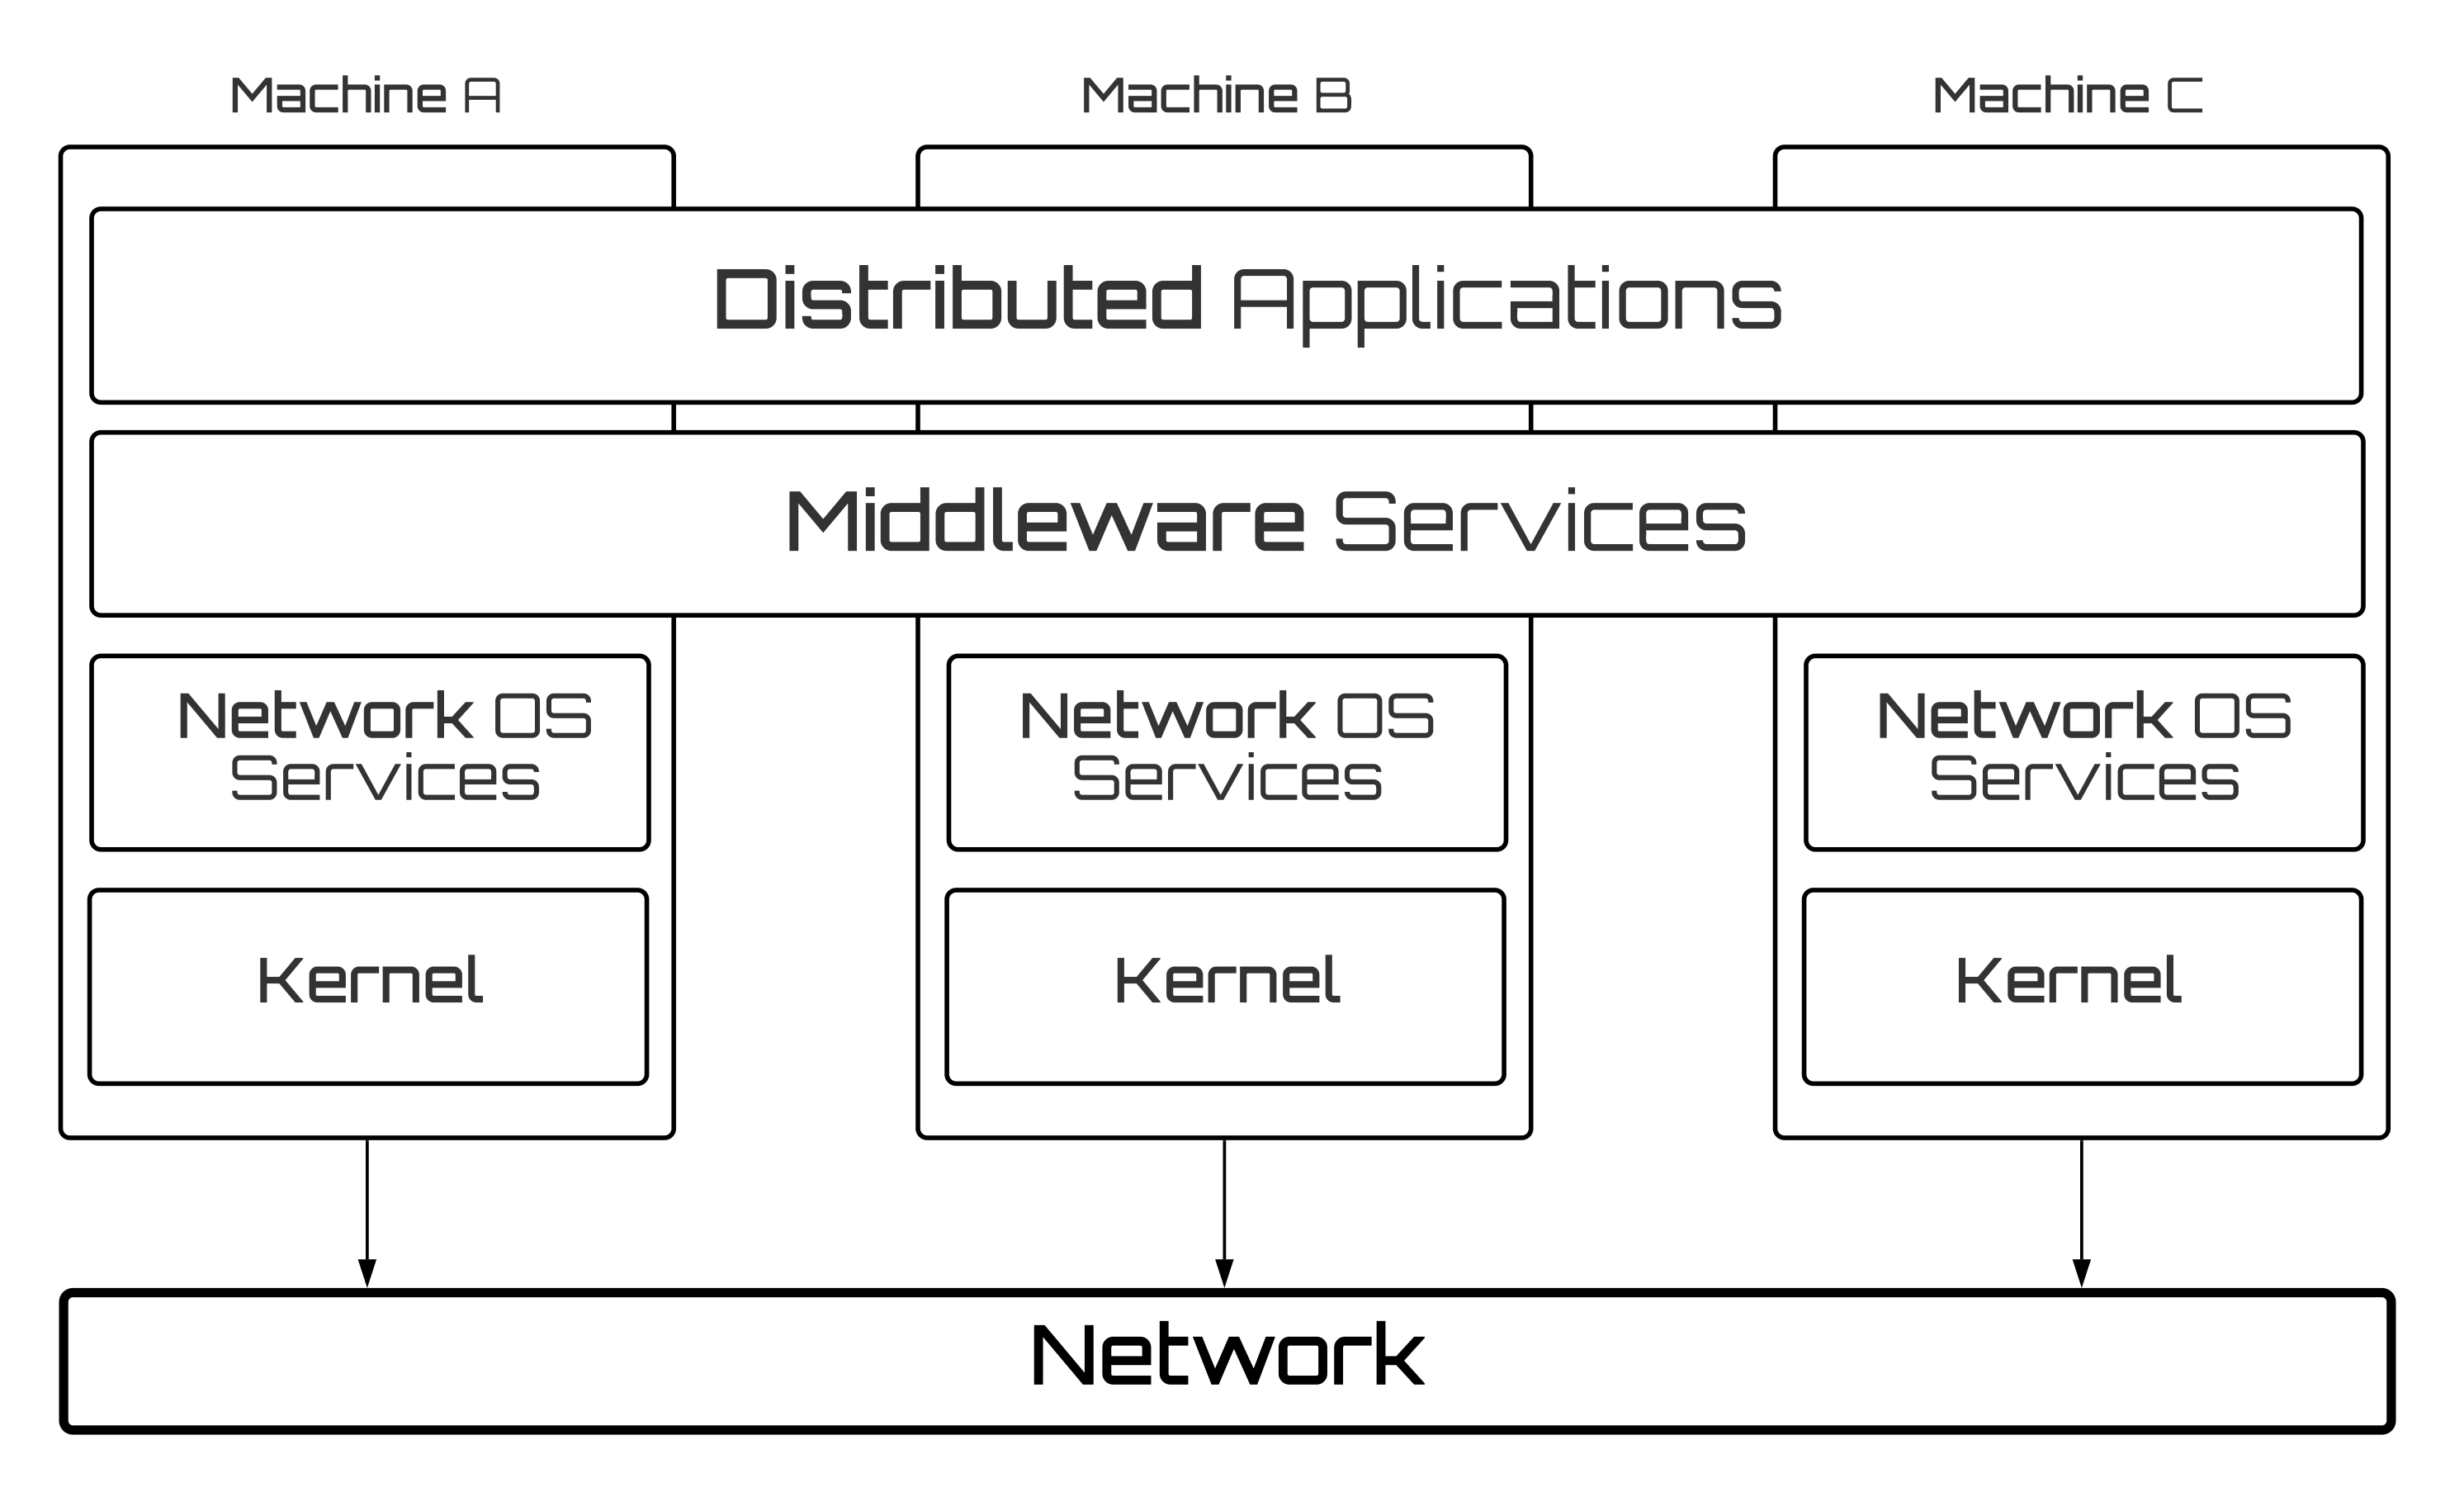
\includegraphics[width=0.8\linewidth,height=6cm]{pictures/midleware_repr_new_new.png}
\caption{Γενική δομή ενός κατανεμημένου συστήματος ως middleware.}
\label{fig:middleware}       
\end{figure}
 
 Τα χαρακτηριστικά που προσδοκήσαμε να αποδώσουμε στο middleware που παράχθηκε, βασίστηκαν στο μοντέλο κατανεμημένων συστημάτων Processor \mbox{Pool} Model (PPM) και την αρχιτεκτονική δικτύου, διαίρει και βασίλευε (Divide and Conquer - Parallel Pipeline). Το πρότυπο PPM απέφερε κατανεμημένη επεξεργασία υψηλής απόδοσης, η οποία θεωρείται απόγονος της κατηγορίας του παράλληλου προγραμματισμού Message-Passing Programming, που προαναφέρθηκε. 

 Το σύνολο των κόμβων διατηρεί σταθερή τη λειτουργία του, ανεξάρτητα με την τοποθεσία και τον τρόπο που διεξάγεται η αλληλεπίδραση μεταξύ του χρήστη και του συστήματος, δηλώνοντας τη συνοχή του. Η αρχιτεκτονική του δικτύου πετυχαίνει μέσω της παραλληλίας που τη διέπει, υψηλές επιδόσεις σε αλγορίθμους, ενώ παρέχεται ως βασικό πρότυπο σχεδίασης δικτύου, μέσω του ZeroMQ. Η ανάλυση των χαρακτηριστικών θα ακολουθήσει παρακάτω. 
 
 \subsection{Αρχιτεκτονική δικτύου}
 
Οι ανάγκες παραλληλίας, ταχύτητας και κλιμάκωσης είναι αυτές που καθόρισαν το μοντέλο που επιλέχθηκε ως βάση για την ανάπτυξη του δικτύου. Όπως και προαναφέρθηκε το μοντέλο που στηριχθήκαμε είναι το Divide and Conquer, το οποίο ονομάζει το ZeroMQ ως Parallel Pipeline. Το πρότυπο αυτό της παραλληλίας δίνει τη δυνατότητα συμμετοχής ακαθόριστου πλήθους συστημάτων-εργατών (worker), οι οποίοι δέχονται εντολές από ένα κεντρικό υπολογιστικό σύστημα (ventilator) και αποστέλλουν τα αποτελέσματα στο τελικό σύστημα συγκέντρωσης αποτελεσμάτων (sink).  
  
\begin{wrapfigure}{r}{0.5\textwidth}
    \centering
    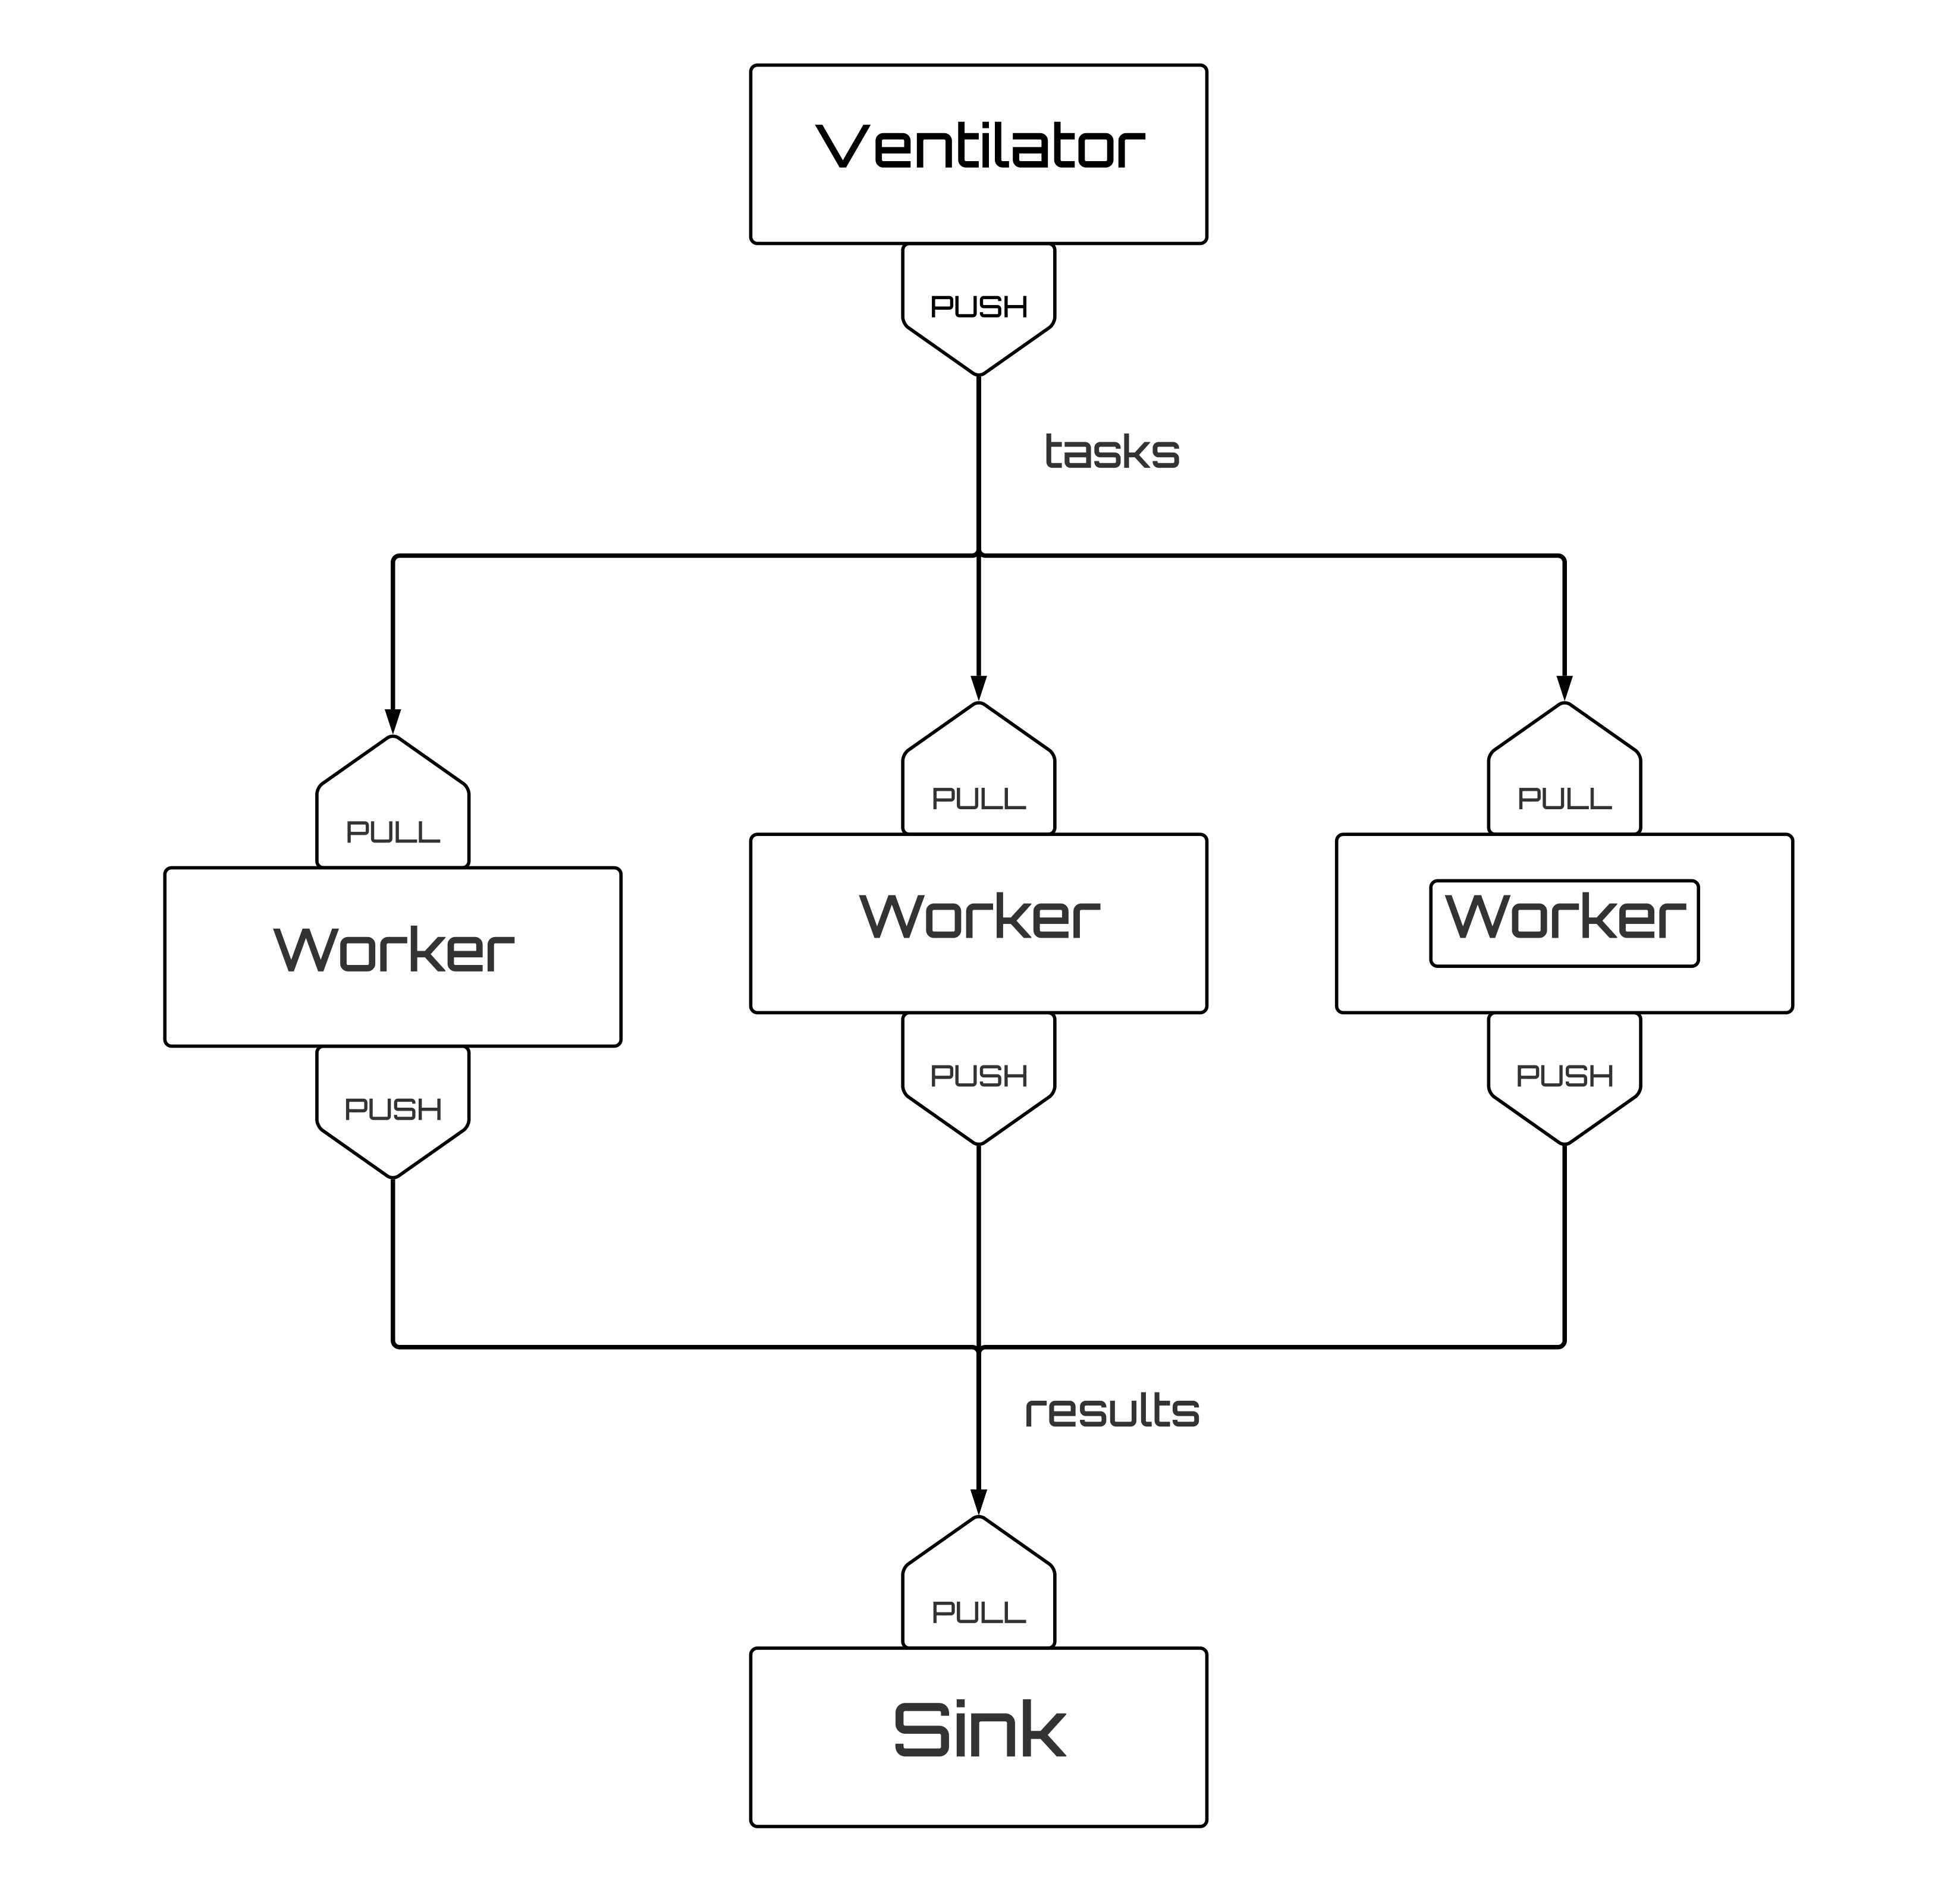
\includegraphics[width=0.4\textwidth, height=7cm]{pictures/ParallelPipeline_new.png}
    \caption{Καθορισμός Parallel Pipeline. } % σύμφωνα με το ZeroMQ.
\end{wrapfigure}  
  
  
% \begin{figure}[!htbp]
% \centering
% 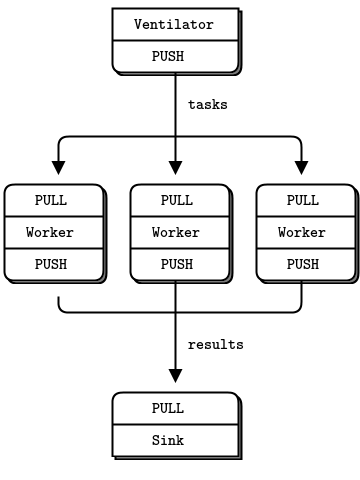
\includegraphics[width=0.8\linewidth,height=12cm]{pictures/ParallelPipeline.png}
% \caption{Καθορισμός Parallel Pipeline σύμφωνα με το ZeroMQ.}
% \label{fig:pipeline}       
% \end{figure}

Το μοντέλο που αναπτύχθηκε στα πλαίσια της εργασίας, αποτελεί μία παραλλαγή του παραπάνω έχοντας μίας βασική προσθήκη και αρκετές εσωτερικές τροποποιήσεις, έτσι ώστε να επιτευχθούν υψηλότερες επιδόσεις. Όπως παρατηρείται και στην απεικόνιση του κατανεμημένου συστήματος παρακάτω, η προσθήκη βρίσκεται στο κεντρικό σύστημα (server) με την προσάρτηση του κόμβου υποβοήθησης (secretary). Ο κόμβος-secretary αφού αλληλοεπιδράσει με τον κόμβο-server, εφαρμόζοντας το πρότυπο αίτημα-απάντηση (request-reply), μεταδίδει με χρήση του προτύπου μετάδοσης-εγγραφής (publish-subscribe) δεδομένα στους κόμβους-worker. Κάθε νέος κόμβος-worker που εισάγεται στο κατανεμημένο σύστημα, ώστε να ενισχύσει με την επεξεργαστική του ισχύ το σύστημα, λαμβάνει πρώτα μηνύματα εγγραφής (subscribe) από τον κόμβο-secretary. 

Οι κόμβοι-worker αφού λάβουν πληροφορίες (info) από τον βοηθητικό κόμβο (secretary), επικοινωνούν με το κόμβο-server εφαρμόζοντας το μοντέλο parallel pipeline. Το σύστημα συγκέντρωσης αποτελεσμάτων είναι ο κόμβος-δοχείο (pot). Οι κόμβοι-worker εκτελούν κάθε διεργασία (task) που λαμβάνουν από τον κόμβο-server, και αποστέλλουν τα αποτελέσματα (result) στο σύστημα συγκέντρωσης αποτελεσμάτων (pot), η διαδικασία αυτή επαναλαμβάνεται έως ότου ο κόμβος κόμβος-server διακόψει τη λειτουργία του. O τελικός κόμβος-pot αφού έχει λάβει στην αρχή τις απαραίτητες πληροφορίες, δέχεται επαναλαμβανόμενα τα αποτελέσματα των κόμβων-worker και στο τέλος ανακοινώνει τη λύση του προβλήματος. Το συνολικό σύστημα που προκύπτει θεωρείται συνεκτικό πληρώντας τις αρχές που διέπουν ένα κατανεμημένο σύστημα. 

\begin{figure}[!htbp]
\centering
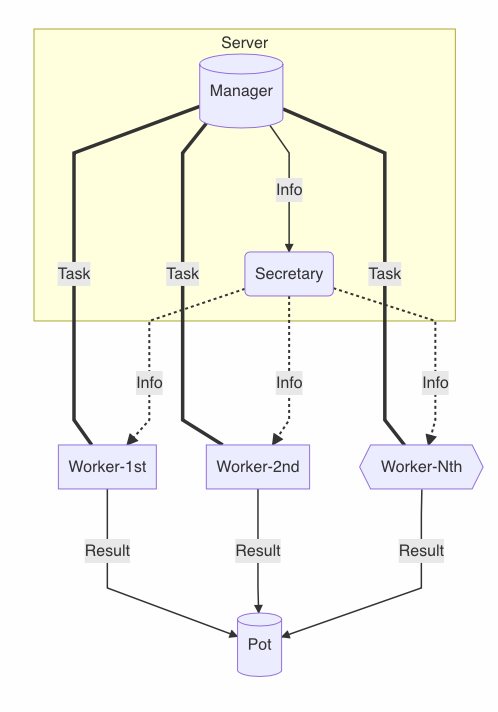
\includegraphics[width=0.8\linewidth,height=12cm]{pictures/PipelineWorkflow.png}
\caption{Διάγραμμα απεικόνισης της γενικής δομής του κατανεμημένου δικτύου.}
\label{fig:workflow}       
\end{figure}

\subsubsection{Δυνατότητες κόμβων}

Το κατανεμημένο σύστημα που παρουσιάζεται, επιτρέπει την απόκρυψη ενδεχόμενων λαθών από τον τελικό χρήστη. Αυτό πρακτικά σημαίνει ότι, τα προγράμματα εφαρμογών μπορούν να συνεχίζουν τις ενέργειές τους παρά την πιθανή αποτυχία κάποιου τμήματος του hardware ή του software, εφαρμόζοντας την αρχή της διαφάνειας αποτυχίας. Το ZeroMQ είναι αυτό που αναλαμβάνει τη διαχείριση μίας τέτοιας κατάστασης αποτυχίας, απομονώνοντας το πρόβλημα, ώστε να μην επηρεάσει το συνολικό σύστημα και επιχειρώντας να επανακάμψει από την κατάσταση σφάλματος, εάν αυτό καθίσταται δυνατόν. 

% Δηλαδή έστω ένας κόμβος-worker που αποτυγχάνει στη διεκπεραίωση της διεργασίας που του έχει ανατεθεί. Το γεγονός αυτό δεν μπορεί να επηρεάσει τη συνολική λειτουργία του κατανεμημένου συστήματος, ενώ παράλληλα ο κόμβος-pot αντιλαμβάνεται την αποτυχία του κόμβου-worker.
%, χωρίς να επηρεασθεί η λειτουργία του. 

Συνεχίζοντας, σύμφωνα με τη διαφάνεια διανομής, ένας χρήστης του κατανεμημένου συστήματος δεν είναι σε θέση να γνωρίζει που πραγματοποιήθηκε ένας υπολογισμός. Επίσης, μία εφαρμογή θα πρέπει να είναι αδιάφορη για το που ακριβώς βρίσκονται αποθηκευμένα τα δεδομένα, ενώ δεν της είναι γνωστό εάν αυτά έχουν αντιγραφεί ή όχι. Η διαφάνεια διανομής εφαρμόζεται και στο εν λόγω σύστημα, καθώς το αρχικό πρόβλημα διασπάται σε υποπροβλήματα μέσω του server. Αυτά διανέμονται στους κόμβους-workers οι οποίοι με τη σειρά τους, δίνουν τα αποτελέσματα τους στο κόμβο-pot. Τέλος, κάποιος κόμβος-worker δεν δύναται να γνωρίζει εάν είναι αυτός που έχει βρει τη λύση του προβλήματος, καθώς αγνοεί ακόμα και το ποιοι άλλοι κόμβοι συμμετέχουν στο σύστημα, πόσο μάλλον το ποια προβλήματα επιλύουν εκείνοι.  \\

%, ούτε μπορεί να γνωρίζει εάν ένας άλλος κόμβος αποτελεί μέλος-worker του συστήματος, πόσο μάλλον για το ποιο υποπρόβλημα επιλύει αυτός. \\ 

\textbf{Η σημασία του κόμβου-secretary} \\

Η προσθήκη ενός επιπλέον κόμβου-secretary προσδίδει περισσότερες δυνατότητες στο κατανεμημένο σύστημα. Αρχικά επιτρέπει την είσοδο νέων κόμβων στο σύστημα σε ακαθόριστο χρόνο, υλοποιώντας το πρότυπο επικοινωνίας publish-subscribe. Κατά αυτόν τον τρόπο αποφορτίζεται ο κόμβος-server από τα αιτήματα νέων worker, ο οποίος μπορεί τώρα αδιάκοπα να επιτελεί τη λειτουργία του. 

Επιπλέον, ο όγκος του κάθε μηνύματος, που αποστέλλει ο κόμβος-server στους κόμβους-worker καθορίζεται πλέον μόνο από τη φύση του προβλήματος, χωρίς να επαναλαμβάνονται γενικές πληροφορίες, παρά μόνο εντολές για τη διεργασία που καλείται να εκτελεσθεί. Οι γενικές πληροφορίες που καθορίζουν το πρόβλημα και είναι αναγκαίες στους νέους κόμβους-worker, μεταδίδονται μόνο μέσω του secretary. Έπειτα, ο κάθε κόμβος-worker τις αποθηκεύει τοπικά, και τις χρησιμοποιεί σε κάθε νέα διεργασία που λαμβάνει από τον κόμβο-server. Το γεγονός αυτό οδηγεί σε δραματικά μικρότερο μέγεθος μηνυμάτων, άρα μικρότερη διάρκεια κωδικοποίησης/αποκωδικοποίησης τους, λιγότερα σφάλματα μετάδοσης και συντομότερη αποστολή τους. Συνεπώς ταχύτερη επικοινωνία μεταξύ server και worker. 

Σε συνδυασμό λοιπόν, με τους αλγορίθμους που αναπτύχθηκαν για τη διάσπαση του προβλήματος σε επιμέρους διεργασίες, η προσθήκη του κόμβου-secretary καθιστά το σύστημα επεκτάσιμο (sclabale). Έτσι, προσφέρεται η δυνατότητα στις εφαρμογές, να επεκτείνουν την κλίμακα τους, χωρίς να υπάρχει αλλαγή στη δομή και στους αλγορίθμους των εφαρμογών.  

% Η αρχή διαφάνειας της κλιμάκωσης του κατανεμημένου συστήματος εφαρμόζεται διαμέσου αυτών.

% Επιπλέον, η παρουσία του κόμβου-secretary μειώνει δραματικά το latency. Αυτό συμβαίνει καθώς δεν υπάρχει κάποιος διαχωρισμός νέων και παλαιών worker, ώστε να απαιτείται η εφαρμογή διαφορετικών μεθόδων που θα αποτελούσαν αιτία αύξησης του συνολικού overhead και καθυστέρησης κατά της διαδικασία δρομολόγησης. Η λειτουργία του κόμβου-server παραμένει σταθερή και επαναλαμβανόμενη καθ' όλη τη διάρκεια λειτουργίας του. 

% χρόνος που απαιτείται για τη μετάδοση ενός κενού μηνύματος μεταξύ συσχετιζόμενων κόμβων.

% Ο κόμβος-secretary αποφορτίζει τον κόμβο-server με ποικίλους τρόπους. Ο όγκος του κάθε μηνύματος που αποστέλλει ο κόμβος-server στους κόμβους-worker καθορίζεται μόνο από τη φύση του προβλήματος χωρίς να επαναλαμβάνονται γενικές πληροφορίες, παρά μόνο εντολές για τη διεργασία που καλείται ο κάθε κόμβος-worker να εκτελέσει. Οι γενικές πληροφορίες που καθορίζουν το πρόβλημα και είναι αναγκαίες στους νέους κόμβους-worker, μεταδίδονται μόνο μέσω του secretary. Έπειτα ο κάθε κόμβος-worker τις αποθηκεύει τοπικά, και τις χρησιμοποιεί σε κάθε νέα διεργασία που λαμβάνει από τον κόμβο-server, που αφορά την επίλυση ενός και μόνου συνολικού προβλήματος. Το γεγονός αυτό οδηγεί σε δραματικά μικρότερο μέγεθος μηνυμάτων, άρα μικρότερη διάρκεια κωδικοποίησης/αποκωδικοποίησης τους, λιγότερα σφάλματα μετάδοσης και συντομότερη αποστολή τους, συνεπώς ταχύτερη επικοινωνία μεταξύ server και worker. 

\subsubsection{Η λειτουργία του προσομοιωτή \lt (Simulator)}  

Στα πλαίσια της εργασίας, αναπτύχθηκε ένα λογισμικό προσομοίωσης της λειτουργίας (simulator) του παραπάνω κατανεμημένου δικτύου, για την επίλυση του προβλήματος εγγύτερου διανύσματος σε πλέγματα. Ο σκοπός που δημιουργήθηκε ήταν η απαίτηση μας να ελέγξουμε τη συμπεριφορά του κατανεμημένου συστήματος σε διάφορες καταστάσεις με διαφορετικές παραμέτρους, αλλά και η δυνατότητα που προέκυψε να εκτελέσουμε επιτυχώς το παραγόμενο λογισμικό σε κατανεμημένο σύστημα με τη χρήση ενός και μόνου πολυπύρηνου συστήματος. Οι πυρήνες του επεξεργαστή του μηχανήματος, προσομοίωσαν τη λειτουργία των διαφόρων τμημάτων του κατανεμημένου συστήματος. Η χρήση του AsyncIO επέτρεψε την προβολή της λειτουργίας όλου του συστήματος από ένα και μόνο τερματικό, εφαρμόζοντας μεθόδους ασύγχρονου \mbox{προγραμματισμού.}  

Ο προσομοιωτής υποστηρίζει Command Line Interface (CLI) σε unix-based συστήματα, όπως MacOS και Linux. Έχει τη δυνατότητα να προσομοιώσει τη λειτουργία κόμβων-worker ανάλογα με τους διαθέσιμους επεξεργαστικούς πυρήνες του συστήματος. Συνεπώς απαιτεί τουλάχιστον τετραπύρηνα συστήματα ώστε να προσομοιώσει τη λειτουργία των τεσσάρων κόμβων, 1 x server, 1 x secretary, 2 x worker και 1 x pot, που θεωρούνται τα ελάχιστα αναγκαία για την εκτέλεση ενός ολοκληρωμένου πειράματος. 

Για τις ανάγκες των πειραμάτων, σε διάφορα συστήματα αλλά και για τον εύκολο διαμοιρασμό του λογισμικού, καθώς θεωρείται ιδιαίτερα απαιτητική η παραμετροποίηση των αναγκαίων προϋποθέσεων για την εκτέλεση του, χρησιμοποιήθηκε η πλατφόρμα ανοιχτού λογισμικού Docker\cite{DockerInPractise}\cite{DockerDeepDive}. Το container docker που παράχθηκε βασίζεται στο λειτουργικό σύστημα Ubuntu, ενώ με εντολές συστήματος οργανωμένες σε αρχεία (Makefiles) γίνεται η μεταγλώττιση (compile) όλων των αρχείων πηγαίου κώδικα (source code) της εργασίας, είτε είναι σε C++, είτε σε Cython, είτε μέσω του Python-Packaging\cite{PythonPackaging} σε Python. 

Σε επίπεδο λειτουργίας, ο προσομοιωτής εκμεταλλεύεται το τοπικό εικονικό δίκτυο (localhost) που παρέχει κάθε σύστημα μέσω του λειτουργικού του συστήματος, ώστε να αποφευχθεί η φυσική διασύνδεση στο δίκτυο. Δεσμεύει ένα πλήθος από πόρτες (ports) του localhost, ανάλογο με αυτό των κόμβων που θα λειτουργήσει. Για τον λόγο αυτό προσφέρεται μέσω του simulator, λειτουργία που κλείνει όλες τις πόρτες που θα χρειαστεί η εφαρμογή για να εκτελεσθεί. Ακόμη μπορεί να καθορισθεί ο ακριβής αριθμός των κόμβων-worker που θα προσομοιωθεί, αρκεί να υποστηρίζεται από την επεξεργαστική μονάδα του συστήματος, όπως επίσης και τα νήματα (threads) που είναι διαθέσιμα προς εκμετάλλευση από τα τμήματα του αλγορίθμου, που εμπεριέχουν παράλληλη επεξεργασία. Επίσης, δίνεται η δυνατότητα στον χρήστη να παραμετροποιήσει με κάθε τρόπο το πρόβλημα που καλείται να επιλύσει το σύστημα, είτε ακόμη να εισάγει ένα πρόβλημα επιλογής του. Τέλος, υποστηρίζει δύο λειτουργίες προσέγγισης της λύσης του προβλήματος, που θα παρουσιαστούν αναλυτικά στη συνέχεια. 
 
\subsection{Παραλληλοποίηση του \lt Schnorr-Euchner Algorithm}

\subsubsection{Φιλοσοφία παραλληλοποίησης}

Ο αλγόριθμος απαρίθμησης δημιουργεί στο παρασκήνιο ένα δένδρο (\mbox{enumeration} tree) το οποίο και προσπελαύνει με τη χρήση του αλγορίθμου διάσχισης γράφων Depth-First Search (DFS), με στόχο την εύρεση του διανύσματος που ικανοποιεί τις απαιτήσεις του προβλήματος. Ο αλγόριθμος DFS όπως προμηνύει και το όνομα του, διασχίζει το δένδρο σε βάθος, δηλαδή κατά μήκος του κάθε κλαδιού, έως ότου καταλήξει σ΄ ένα κόμβο-φύλλο της δενδρικής δομής, όπου ενδεχομένως αποτελεί υποψήφια λύση του προβλήματος. Η ιδέα που στηρίχθηκε η παραλληλοποίηση του αλγορίθμου Schnorr-Euchner έγκειται στην παραλληλοποίηση της αναζήτησης στο δένδρο απαρίθμησης, δηλαδή του DFS. 
 
 %  - ακυκλικός συνδεδεμένος γράφος -

Η παραλληλοποίηση στηρίζεται στην απλή ιδέα, της διάσπασης του δένδρου απαρίθμησης σε υποδένδρα. Η αρχική δενδρική δομή διασπάται σε μικρότερες, οι οποίες με τη σειρά τους διαμοιράζονται σε κατανεμημένα ανεξάρτητα συστήματα. Σε κάθε σύστημα επαναλαμβάνεται η διαδικασία διάσπασης. Ανάλογα με τους διαθέσιμους πόρους του συστήματος διασπάται το υποδένδρο σε μικρότερα, ώστε να εκτελεσθεί ταυτόχρονα σε κάθε δένδρο η αναζήτηση του μικρότερου διανύσματος. Ο τρόπος με τον οποίο εφαρμόζεται η διάσπαση σε υποσύνολα-υποδένδρα εκμεταλλεύεται την πρόταση του αλγορίθμου KFP, για τον ορισμό των διαστημάτων $ I_k $. 
 
$$ I_k = \Bigg[- \sum_{i=n+2-k}^n μ_{i,n+1-k} u_i - \sqrt{\frac{R^2 - \sum_{j=n+2-k}^n l_j}{\| \bm b_{n+1-k}^* \|}}, 
- \sum_{i=n+2-k}^n μ_{i,n+1-k} u_i + \sqrt{\frac{R^2 - \sum_{j=n+2-k}^n l_j}{\| \bm b_{n+1-k}^* \|}} \Bigg] $$
 
Έπειτα, εφαρμόζεται ο αλγόριθμος Schnorr-Euchner, σύμφωνα με τον οποίο η αναζήτηση στα διαστήματα $I_k$ ξεκινάει από τη μέση του διαστήματος. 

\subsubsection{Δυνατότητες υλοποίησης}

Η μέθοδος με την οποία γίνεται η διάσπαση του δένδρου μπορεί να διαφέρει, γι' αυτό και στην παρούσα εργασία υλοποιήθηκαν δύο προσεγγίσεις. Η πρώτη στηρίζεται στο πλήθος των διεργασιών που θεωρείται επιθυμητό να διασπασθεί το πρόβλημα, ενώ η δεύτερη στην ιδέα της διάσπασης του προβλήματος, αφού πρώτα υπολογισθούν τα διαστήματα για κάποιο συγκεκριμένος βάθος του δένδρου απαρίθμησης. Οι δύο αυτές παραλλαγές ισοδυναμούν με τις δύο διαφορετικές λειτουργίες του Simulator που αναφέρθηκαν στην προηγούμενη ενότητα. 

Η διάσπαση του δένδρου βάσει του επιθυμητού πλήθους διεργασιών, έχει καλή εφαρμογή όταν έχουμε γνώση του ακριβή αριθμού των κόμβων-worker, καθώς τότε ο διαμοιρασμός μπορεί να είναι ακριβής. Έτσι αποφεύγεται η εμφάνιση του σύνηθες προβλήματος, κατά το οποίο απομένει να εκτελείται μία περίσσεια διεργασία ενώ τα υπόλοιπα συστήματα έχουν ολοκληρώσει την επεξεργασία τους. Κάτι τέτοιο θα μπορούσε να οδηγήσει ακόμα και σε διπλασιασμό της εκτέλεσης του συστήματος. Φυσικά υπάρχουν ποικίλες λύσεις στο πρόβλημα αυτό, όπως το dynamic-scheduling ή ο αλγόριθμος Round Robin, αλλά στη δική μας περίπτωση αυξάνουν αισθητά την πολυπλοκότητα. Συνεπώς, καταλήξαμε πως εάν γνωρίζουμε τον αριθμό των κόμβων-worker, επιλέγουμε το πλήθος των διεργασιών έτσι ώστε να είναι ακέραιο πολλαπλάσιο του πλήθους των κόμβων-worker, αυξάνοντας ενδεχομένως σε κάποιες περιπτώσεις τις απαιτήσεις μερικών διεργασιών. Πιο αναλυτικά, ενώ υπό ιδανικές συνθήκες τα υποσύνολα (υποδένδρα) που διαμοιράζονται έχουν τον ίδιο αριθμό στοιχείων, σε περιπτώσεις όπως την προαναφερθείσα διαφέρουν, ώστε να μην υπάρχει πλεόνασμα, γι' αυτό και οι απαιτήσεις των διαμοιραζόμενων διεργασιών δεν είναι ισοδύναμες.  

Η έναρξη της παράλληλης επεξεργασίας αφού προϋπολογισθούν κάποια διαστήματα $ U_n,U_{n-1},...,U_k $ όπου $ k \in \mathbf{Z} $ είναι η δεύτερη λειτουργία που υλοποιήθηκε. Σύμφωνα μ’ αυτή τη λειτουργία μπορούν να κλαδευτούν κάποια υποδένδρα τα οποία δεν θα οδηγούσαν σε κάποια λύση, γι’ αυτό και συνίσταται η επιλογή του κατάλληλου $k$ μετά από ανάλογο πειραματισμό, (σ’ αυτή τη προσέγγιση θα μπορούσαν να εφαρμοσθούν τεχνικές Machine Learning για την επιλογή του $ k $). Ο ακέραιος αριθμός $ k $ συμβολίζει το βάθος που θα προσπελαθεί στο δένδρο απαρίθμησης έως ότου διασπασθεί σε υποδένδρα. Το πλήθος των διεργασιών που προκύπτει διαφέρει ανάλογα την περίπτωση, αλλά η φιλοσοφία διαχωρισμού τους είναι η ίδια μ' αυτή που εφαρμόζεται στην προηγούμενη λειτουργία. 

\subsubsection{Ανάλυση συστήματος}

Το κατανεμημένο σύστημα παράλληλης επεξεργασίας για $ m $ το πλήθος κόμβους-workers και $ n $ αριθμό νημάτων-threads σε κάθε κόμβο-worker, μπορεί να εκτελέσει παράλληλα, $ m*n $ διεργασίες. Η λειτουργία του συστήματος αυτού, παρουσιάζεται αναλυτικά στο διάγραμμα \ref{fig:system}. 

\begin{figure}[!htbp]
\centering
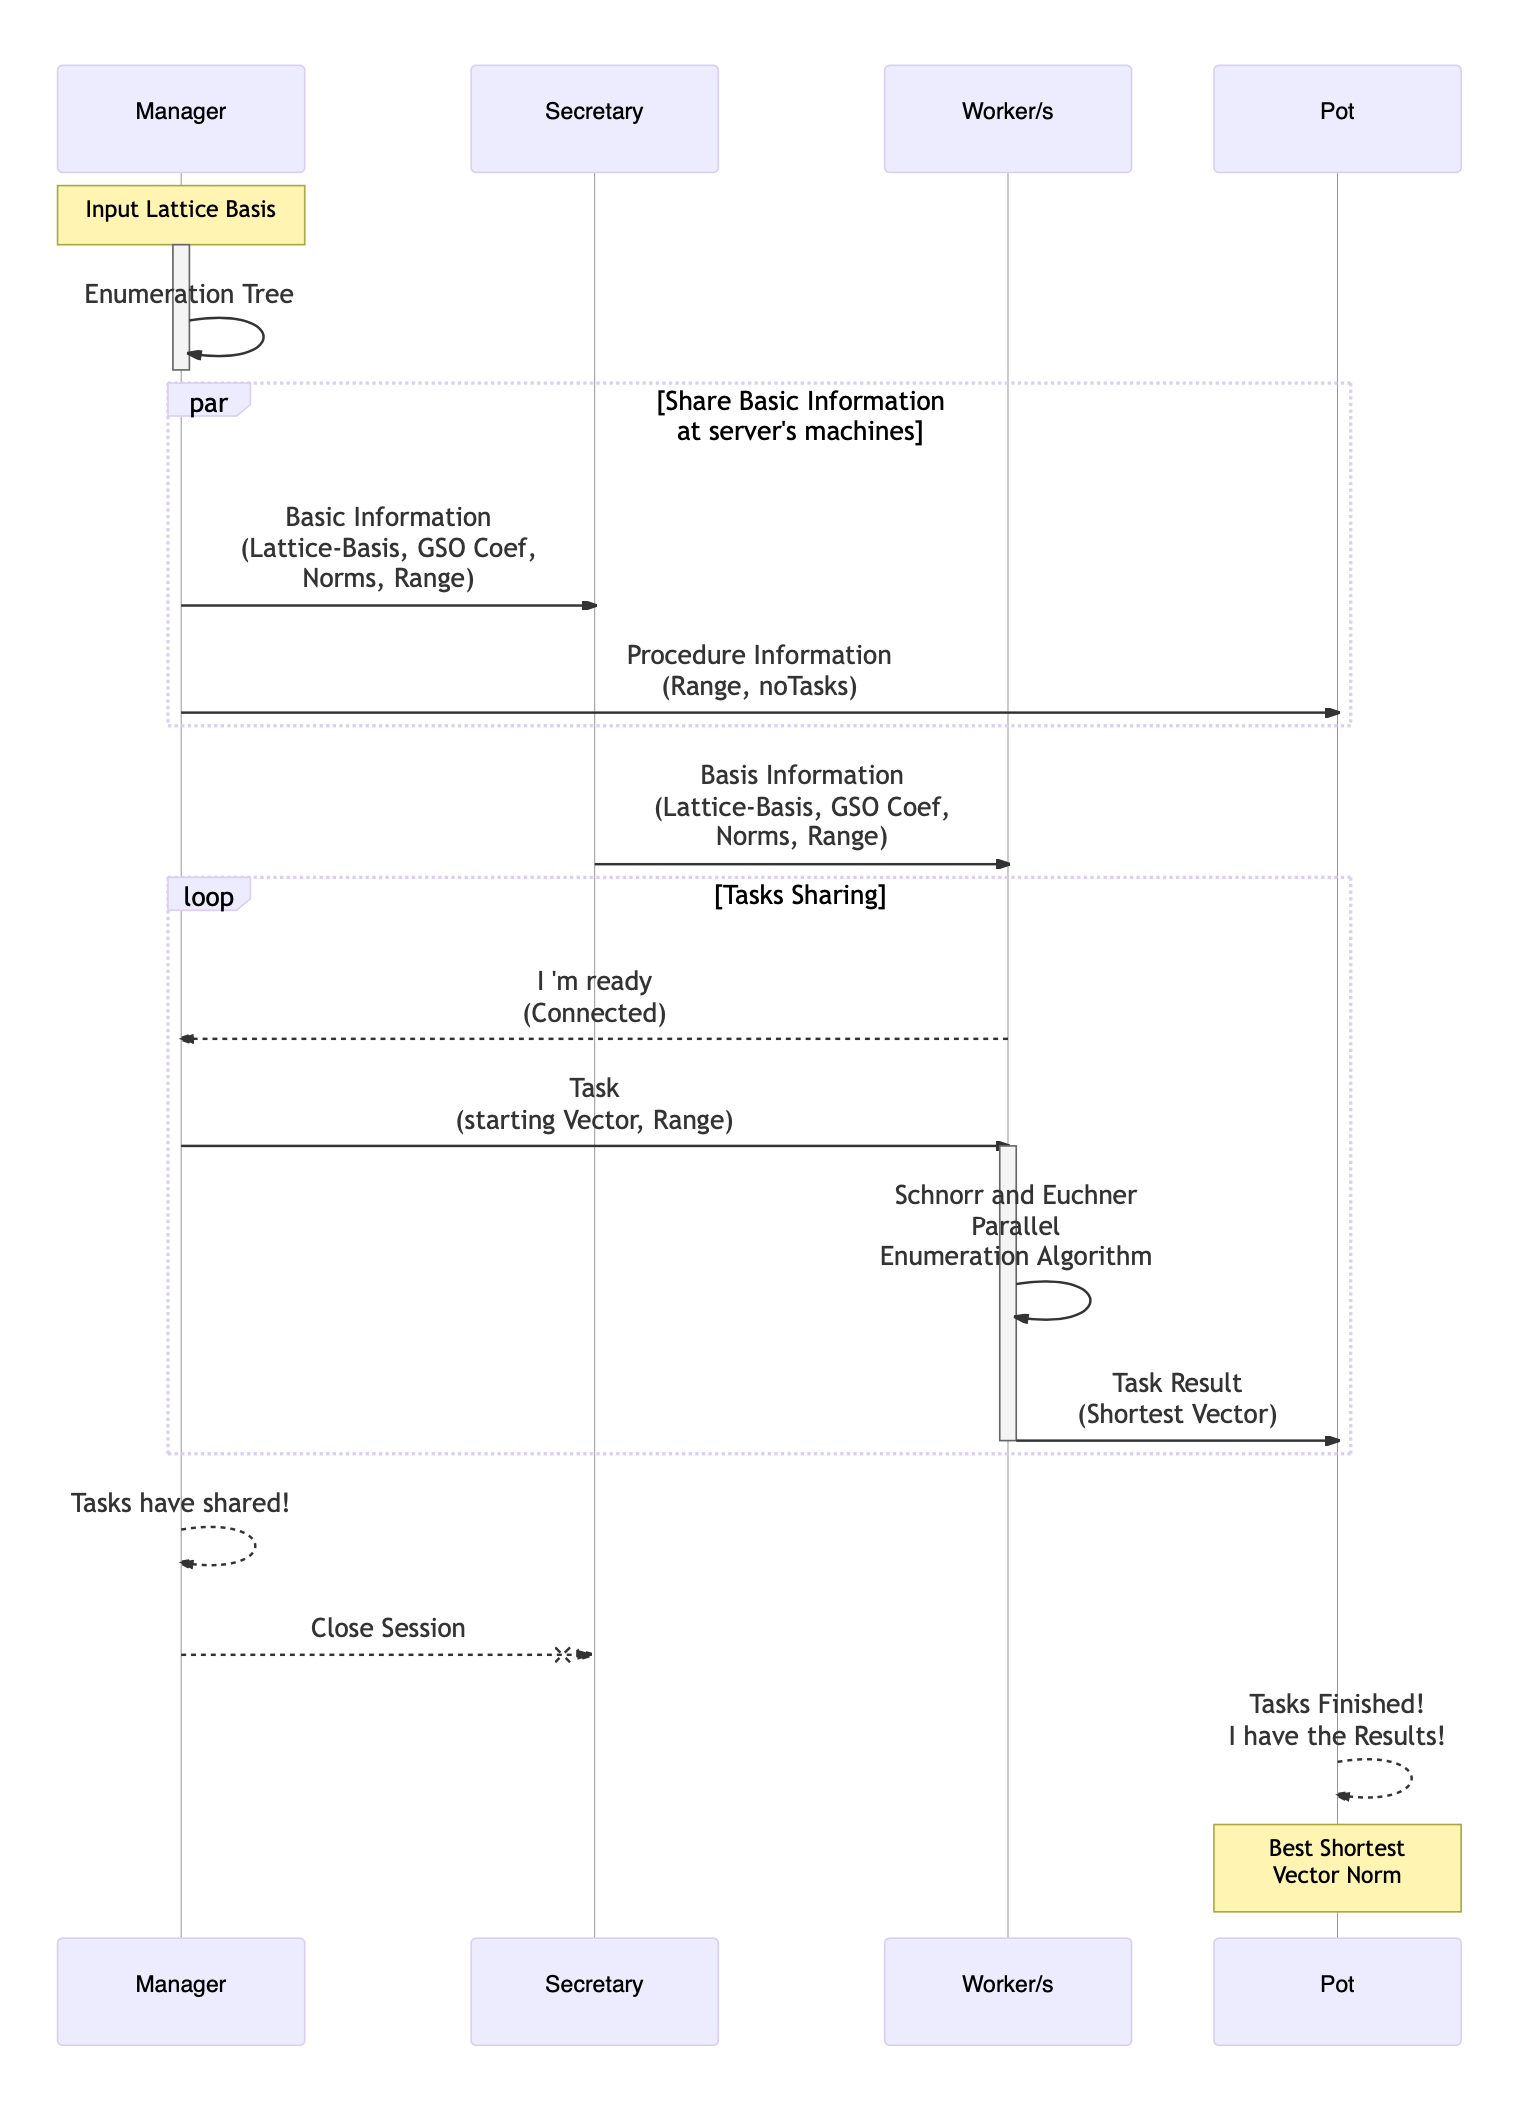
\includegraphics[width=0.8\linewidth,height=16cm]{pictures/SystemAnalysis.png}
\caption{Λειτουργία του κατανεμημένου συστήματος.}
\label{fig:system}       
\end{figure}

Έπειτα, στους αλγορίθμους που ακολουθούν παρουσιάζουμε τις μεθόδους που ακολουθήθηκαν για την επίτευξη της παραλληλίας στο συνολικό σύστημα. Η λειτουργία της διάσπασης λαμβάνει χώρα στον server node όπου δημιουργείται ένα δέντρο απαρίθμησης μέσω του αλγορίθμου \emph{4.1}, το οποίο διασπάται σε επιμέρους κλαδιά (συνδεδεμένη λίστα), που συμβολίζουν τις διεργασίες. Στη συνέχεια διαμοιράζονται σε καθέναν από τους worker nodes. Οι worker nodes αφού λάβουν τις διεργασίες, σύμφωνα με τον αλγόριθμο \emph{4.2}, τις διασπούν σε υποδιεργασίες  οι οποίες εκτελούνται παράλληλα στον επεξεργαστή του συστήματος. Κύριο μέλημα είναι καμία υποδιεργασία να μην παρεμβαίνει στο χώρο αναζήτησης κάποιας άλλης, ώστε να μην υπάρχει σπατάλη επεξεργαστικού χρόνου, αυτό επιτυγχάνεται με τον αλγόριθμο \emph{4.3}, παραλλαγή του αλγορίθμου των Schnor και Euchner\cite{journals/mp/SchnorrE94}.

\begin{algorithm}[h] \label{split}
\SetAlgoLined

{\bf Input:} $ μ, Β^*, n $  \\
{\bf Output:} Tree branches. \\

\hfill

$ B^*_i = \| b^*_i \|^2, μ = GSO(B) $ \quad \emph{\#Calculate Gram-Schmidt Orthogonalization} \\

$ tree = new \; Tree() $ \\
$ x\_vector = new \; Vector(n) $  \quad \emph{\# Fill with zeros} \\

\emph{\# Calculate $ I_k $} \\
$ upper\_bound = find\_range\_KFP(M, B^*, n, tree.height+1, x\_vector).upper\_bound $

$ tree.new\_root\_node(upper\_bound, n, x\_vector) $ \\
$ BFS = tree.iterator.begin() $ \\
$ total\_range = 1 $ \\
$ expression = distribution\_mode.expression() $ \emph{\# modes: [via\_Nodes, via\_Depth]}\\
\While{$ expression(total\_range)$} { 
    $ parent = bfs() $ \\
    $ height = parent.depth + 1 $ \\
    \If{$ n < height $}{
        \textbf{break}
    }
    $ index = n - height $ \\
    \For{$int \; i=0; \; i\leq parent.upper\_bound; \; i++$} {
        $ new\_x\_vector = parent.x\_vector $ \\
        $ nex\_x\_vector[index] = i$ \\
        $ new\_upper\_bound = find\_range\_KFP(height, new\_x\_vector).upper\_bound $ \\ 
        $ tree.new\_node(new\_upper\_bound, n, new\_x\_vector, index) $ \\
    } 
    $ total\_range += parent.upper\_bound $ \\
    $ BFS.next() $ \\

} % end of while
\textbf{return} $ tree.get\_branches() $

\caption{Sever-Node: Enumeration Tree for Distributed Operation}
\end{algorithm}





\begin{algorithm}[h] \label{split-worker}
\SetAlgoLined

{\bf Input:} $ server\_msg, no\_threads $ \\
{\bf Output:} S \\

\hfill

$ μ = server\_msg.get\_GSO\_Coefficients() $ \\
$ B^* = server\_msg.get\_B\_norms2() $ \\
$ n = server\_msg.get\_size() $ \\
$ R = server\_msg.get\_R() $ \\
$ branch = server\_msg.get\_process() $ \\


$ x\_vector = branch.x\_vector $ \\

$ index\_border = branch.index $ \qquad \qquad \emph{\#constant}\\
\If{$ index\_border == 0 $}{
    \textbf{return} $ x\_vector $
}
$ range = branch.upper\_bound + 1 $ \qquad \emph{\#[0, branch.upper\_bound]} \\ 
$ no\_tasks = range // threads $ \qquad \emph{\#integer\ division} \\
$ balance = range \% threads $ \qquad \emph{\#modulo} \\

\If{$ no\_tasks == 0 $}{
    $ no\_threads = balance $
}
$ x\_parallel = new Array(n,\ no\_threads) $ \\
\textbf{parallel}
\For{$ t=0,\ t< no\_threads,\ t++ $}{ 
$ copy(x\_parallel[t],\ x\_vector,\ n)$
}

$ S = new \ ParallelHeap() $ \\
\textbf{parallel}
\For{$ t=1,\ t< no\_threads,\ t++ $}{
$ extra\_task = (t+balance-no\_threads)*((t+balance)>=no\_threads) $ \\
$ upper\_bound = no\_tasks*t -1 + extra\_task  $ \\
$ lower\_bound = upper\_bound + 1 - no\_tasks - ((t+balance)>=no\_threads) $\\

$ S = S \cup \{ Bounded\_SchnorrEuchner(μ,\ Β^*,\ n,\ R,$ \\ $ \qquad x\_parallel[t\_id],\ index\_border,\ lower\_bound, upper\_bound)\} $
}



\textbf{return} $ S $

\caption{Worker-Node: Schnorr-Euchner Parallel Operation}
\end{algorithm}





\begin{algorithm}[h] \label{bounded}
\SetAlgoLined

{\bf Input:} $μ, Β^*, n, R, x, i_{border}, lower\_bound, upper\_bound $,  \\
{\bf Output:} S \\

\hfill

$ \bm c = (c_i) \gets \bm 0_n, l = (l_i) \gets \bm 0_n $ \\
$ Δx \gets (1, \bm 0_{n-1}), Δ^2x \gets(1,(-1)_{n-1}), suml_i \gets 0, S = \emptyset, i \gets 0, S \gets []) $ \\

\While{$ i < i_{bound} $} { 

    $ c_i \gets - \sum_{j=i+1}^{n-1} x_jμ_{ji}$ \\
    $ l_i \gets B_i(x_i - c_i)^2 $ \\
    $ sumli \gets \sum_{j=i}^{n-1}l_j $ \\
    
    \If{$ sumli \leq R^2 $ and $ i=0 $}{
        $ S \gets S \cup \{ \sum_{j=0}^{n-1} x_j b_j \} $ \\
    }
    \If{$ sumli \leq R^2 $ and $ i>0 $}{
            $ i = i - 1 $ \\
            $ c_i \gets - \sum_{j=i+1}^{n-1} μ_{j,i} x_j $ \qquad \emph{\# center of interval $ I_{n+1-i}$} \\
            $ x_i \gets \lceil c_i \rfloor $ \\
            $ Δx_i \gets 0 $ \\
            \eIf{$ c_i < x_i $}
            {$ Δ^2x_i \gets 1 $ }
            {$ Δ^2x_i \gets -1 $}
    }
    {
    \eIf{$ i==i_{border} \ OR \ ( i==i_{border}-1 \ AND \ ( x[i] < lower\_bound \ OR \ x[i] > upper\_bound ))$}{
    \textbf{break}
    }
    {
    $ i \gets i + 1 $ \\
    $ Δ^2x_i \gets - Δ^2x_i $ \\
    $ Δx_i \gets -Δx_i +Δ^2x_i $ \\
    $ x_i \gets x_i + Δx_i $ \\
    \If{$ i==i_{border}-1 \ AND \ ( x[i] < lower\_bound \ OR \ x[i] > upper\_bound )$}{
    \textbf{break}
    }
    
    }
    
    }

} % end of while
\textbf{return} $ S $

\caption{Bounded Schnorr-Euchner Enumeration Algorithm}
\end{algorithm}
